
\phantomsection
\pagestyle{plain}

\begingroup

\let\clearpage\relax
\let\cleardoublepage\relax
\let\cleardoublepage\relax

\begin{interludeenv}

\renewcommand\thefigure{\theinterludes-\arabic{figure}}
\setcounter{figure}{0}

\interlude{A Primer to Mechanistic, Individual-based Models as Conceptual Tools in Evolutionary Ecology}\label{box:demos}

\noindent \textbf{Pratik R. Gupte}

\medskip

\noindent {\large{$\Delta$}} {\footnotesize This small demonstration accompanies the Introduction in a submission to \emph{Ecology Letters}.}

\medskip

Here, I present a prototype of the models I outlined in the Introduction, in order to show how my approach differs from approaches used thus far.
I show that considering movement as the outcome of evolved preferences for locally available cues leads to very different ecological outcomes when compared to mainstream frameworks such as random walks and optimal local movement.
These differences can be important when such models are used as baselines against which to compare patterns observed from empirical animal tracking data, or to make predictions for how key ecological processes --- such as the transmission of pathogens or culture --- occur in animal populations \parencite{cantor2021}.
Here I focus on movement strategies following \textcite{bastille-rousseau2019}, which are among the behavioural strategies of individuals, and which may also facilitate or constrain which other behavioural strategies individuals can employ \citep{nathan2008a,spiegel2017}.

I compare ecological outcomes of four movement scenarios of a model with the same ecological processes.
In my model, 200 individuals inhabit a landscape of 30 square units, which also contains 450 discrete food items (see Fig.~\ref{fig:demo_schematic}).
Food items are patchily distributed to form distinct clusters (N = 30, 15 items per cluster).
For the sake of simplicity, individuals choose only a movement direction, and have the same movement distance of 1 distance unit (like a king in chess; see Fig.~\ref{fig:demo_schematic}).
Individuals can perceive food items ($F$) and other individuals at locations 1 distance unit away.
When individuals perceive a food item, they pick it up and handle it for 5 time-steps until they can gain its energetic benefit \citep{ruxton1992,gupte2021a,gupte2022c}; I call such individuals `handlers' ($H$).
While individuals are handling an item, they are immobilised.
Individuals compete with each other exploitatively and an item once picked up by an individual is unavailable to its neighbours; these individuals continue searching for food, and I call them `non-handlers' ($N$).
Items regenerate at the same location after a fixed number of timesteps, which I call the regeneration time ($T_R$; default = 100), and while an item is regenerating, it cannot be sensed by nearby individuals.
Individuals have a lifetime of 400 timesteps, over which they forage and move over the landscape.
The model's four scenarios differ in their implementation of individual movement.

\begin{figure}[!h]
    \centering
    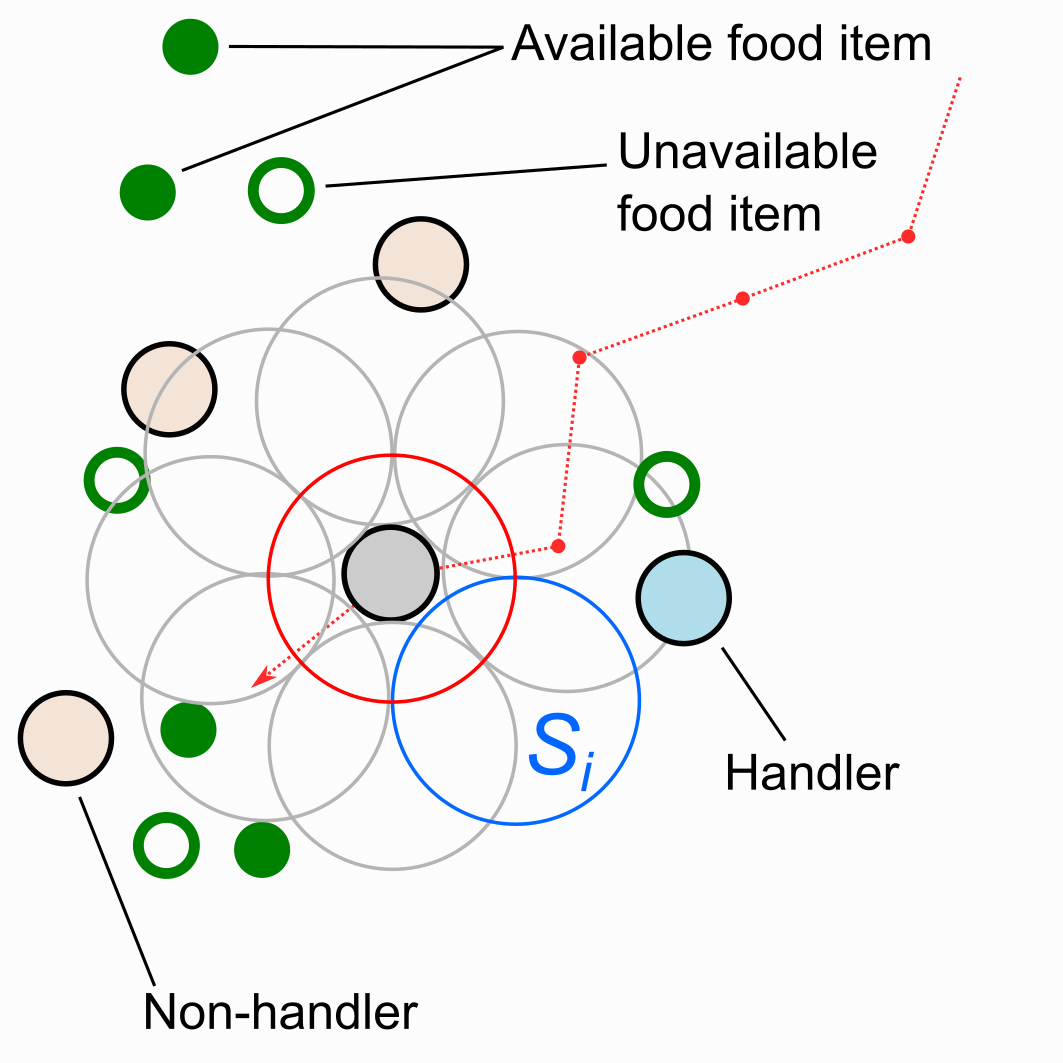
\includegraphics[width=0.9\linewidth]{figures/introduction/fig_schematic.png}
    \caption{
        \textbf{Schematic for a conceptual model of individual foraging movement as a series of discrete steps in continuous space, with movement steps selected based on individual preferences for environmental cues.} 
        In this model, individuals search for patchily distributed food items (\textbf{green circles}), which may be immediately available (\textbf{filled green circles}; \emph{F}), or may be available only in the future (\textbf{open green circles}). 
        Individuals can sense only available items, and not unavailable ones. However, as food items are clustered, available items are a good indirect indicator of where resource clusters are, and where items may become available in the future. 
        Individuals can also sense other foraging individuals, and can sense whether they have successfully found, and are handling, a food item (handlers; \textbf{blue circles}), or whether they are unsuccessful foragers still searching for food (non-handlers; \textbf{filled pink circles}; \emph{N}). 
        To decide where to move, individuals sample their environment for these three cues (\emph{F, H, N}) at their current location (\textbf{red circle}), and at a number of locations around themselves (\textbf{large open grey circles}; here, 8 locations). 
        When the sensory range is relatively large there is some small overlap in samples. 
        Individuals take their next step by assigning each potential direction a \emph{suitability}, $S = s_FF + s_HH + s_NN + \epsilon$, where the coefficients $s_F, s_H, s_N$ are individual weights for environmental cues (`cue preferences'), and $\epsilon$ is a small error term that helps break ties between locations.
        The individual moves in the direction of highest suitability the cue weights fully determine the movement of an individual. Then say that the cue weights can be implemented as heritable and, hence, evolvable properties.
    }
    \label{fig:demo_schematic}
  \end{figure}

\subsection*{Scenarios in the Model}

In \textit{scenario 1}, individuals perform a random walk, and have a uniform probability of either remaining in their current location, or moving in a direction chosen from among eight locations within 1 distance unit (see Fig.~\ref{fig:demo_compare}A); here, movement is independent of local cues.
In \textit{scenario 2}, individuals move in a way that is considered locally optimal in foraging ecology \citep{stephens2019,scherer2020}.
Each individual assesses local cues at its current location, and eight surrounding locations --- the number of available food items ($F$), and the number of potential competitors ($N + H$) --- and moves to the location with the highest expected intake, which is given by $(F / (N + H + 1)) + \epsilon$; $\epsilon$ is a small error term.
I initially contrast these two scenarios to show how adding suitability-based decision making to individual movement can affect the outcomes of movement individual-based models.

Locally optimal movement models are often labelled mechanistic as they include environmental cues in decision making \citep[e.g.][]{scherer2020}, yet the expected payoff of a location is strongly influenced by the functional response of intake in relation to competitors.
Such implementations make the implicit evolutionary assumption that all individuals individuals can `sense' the fitness revenue per location and then move in the direction of fitness increase.
% However, the functional responses commonly used in foraging theory are often modelled on empirical data, and as such may not be properly generalisable to other eco-evolutionary contexts, nor sufficient to capture the mechanistic links between individuals' social environment, their behavioural decisions, and the consequences for intake.
I showcase a more mechanistic way in which individuals can determine their optimal step when making foraging movements, which is to have distinct preferences for local cues (food items and potential competitors).
These preferences are similar to the coefficients of habitat- and step-selection functions \citep[][]{fortin2005,thurfjell2014,manly2002}.

In my model's \textit{scenario 3}, individuals assesses local cues --- the number of available food items ($F$), and the number of potential competitors ($N + H$) --- at eight locations around themselves, and move to the location with the highest assessed suitability: $S = s_FF + s_C(N + H) + \epsilon$.
Here, $s_F$ and $s_C$ are inherited \textit{movement preferences} for food items and potential competitors respectively, and can take any positive or negative numeric values; $\epsilon$ is a small error term.
It is the relative contribution of $s_F$ and $s_C$ that determines individuals' \textit{movement strategy} \parencite[similar to the behavioural hypervolume of][]{bastille-rousseau2019}.
I initialised the populations to have a broad range of movement strategies, so that it contained individuals with different combinations of preferences and avoidances of either food items or competitors.
This assumption matters, as it speeds up initial evolution by orders of magnitude. 
This method is useful for obtaining a first `quick' overview of the evolutionary outcome, but it is advisable to check whether the same outcome is achieved when starting with a monomorphic population with zero cue weights.

In my evolutionary approach, I am more interested in cue weights (and strategies) that have evolved subject to natural selection.
Since individuals inherit their cue weights from their parents, and successful parents produce more offspring (lifetime intake is the proxy for `fitness'), successful movement strategies are transmitted to more offspring and will thus spread in the population \parencite[an expectation from the replicator equation:][]{hofbauer1988}.
To examine which movement strategies evolved, I added an evolutionary component to the model: over 100 generations, individuals reproduce, passing on their preferences ($s_F$, $s_C$) to their offspring.
The preference values undergo random, independent mutations with a probability $p$ = 0.01, and with a mutation step size drawn from a Cauchy distribution with a scale of 0.01.
Consequently, most mutations are small, but larger mutations do occasionally occur.

For simplicity, I assume fixed population size, discrete, non-overlapping generations, asexual reproduction, and haploid individuals.
I implemented large-scale natal dispersal, such that individuals are typically initialised (`born') within a standard deviation of 10 units of their parents (see \cite{travis1999} for a consideration of how dispersal itself evolves).
This makes scenario 3 relatively similar to the random initialisation of individual positions in scenarios 1 and 2.
These modelling choices must be explicitly implemented in simulation models' code, bringing the assumptions of classical models --- treated as received wisdom and hence ignored --- to the fore.

A key feature of individual-based simulation models is their ability to incorporate great amounts of ecological detail \citep{deangelis2019}.
With a simple extension to scenario 3, I show how to add biologically relevant details to models, and how these details can affect model outcomes.
Foraging can be a form of public information, serving as an indirect cue of the presence of resources, and furthermore, helping distinguish between individuals that are \textit{immediate} competitors (here, non-handlers), and those which are only future potential competitors \citep[][; here, handlers]{dall2005,giraldeau2018,beauchamp2008,beauchamp2013}.
Thus in my \textit{scenario 4}, I allow individuals to sense the handling status of nearby potential competitors, and to have separate heritable preferences for handlers ($sH$) and non-handlers ($sN$).
Individuals assess the suitability of locations as $S = s_FF + s_HH + s_NN + \epsilon$; $\epsilon$ is a small error term.
I implemented the same evolutionary and dispersal assumptions as in scenario 3.

\subsection*{Comparing Scenario Outcomes}

As expected, optimally moving scenario 2 individuals had a higher per-capita intake than randomly moving scenario 1 individuals (Fig.~\ref{fig:demo_compare}).
Individuals with higher intake should be expected to move less, as my model --- in line with foraging ecology theory \citep{charnov1976} --- explicitly considers a tradeoff between movement and intake.
Specifically, the tradeoff is that when an individual is handling, it cannot move towards areas of higher future expected intake, and if an individual moves into locations where there are no food items, it loses out on intake.
Individuals following a locally optimal strategy moved \textit{more} than random walkers (Fig.~\ref{fig:demo_compare}), a clear confirmation of the expectation that such a strategy is more efficient than random walking (i.e., more food for less movement).
Nonetheless, individuals in both scenarios had very similar numbers of spatial associations with other individuals (Fig.~\ref{fig:demo_compare}, Fig.~\ref{fig:demo_networks}).
Overall, this comparison demonstrates the importance of active decision making in animal movement, and suggests why animals have evolved sophisticated sensory apparatuses to gather information from their environment \citep{avgar2013,berger2022,mann2021,swain2021}.
Such evolution is likely to be strongly dependent on fine-scale ecological conditions, primarily the \textit{availability} of information in the environment, as well as the energetic cost of evolving and maintaining sensory capabilities \citep{swain2021}.

\begin{figure}[!h]
    \centering
    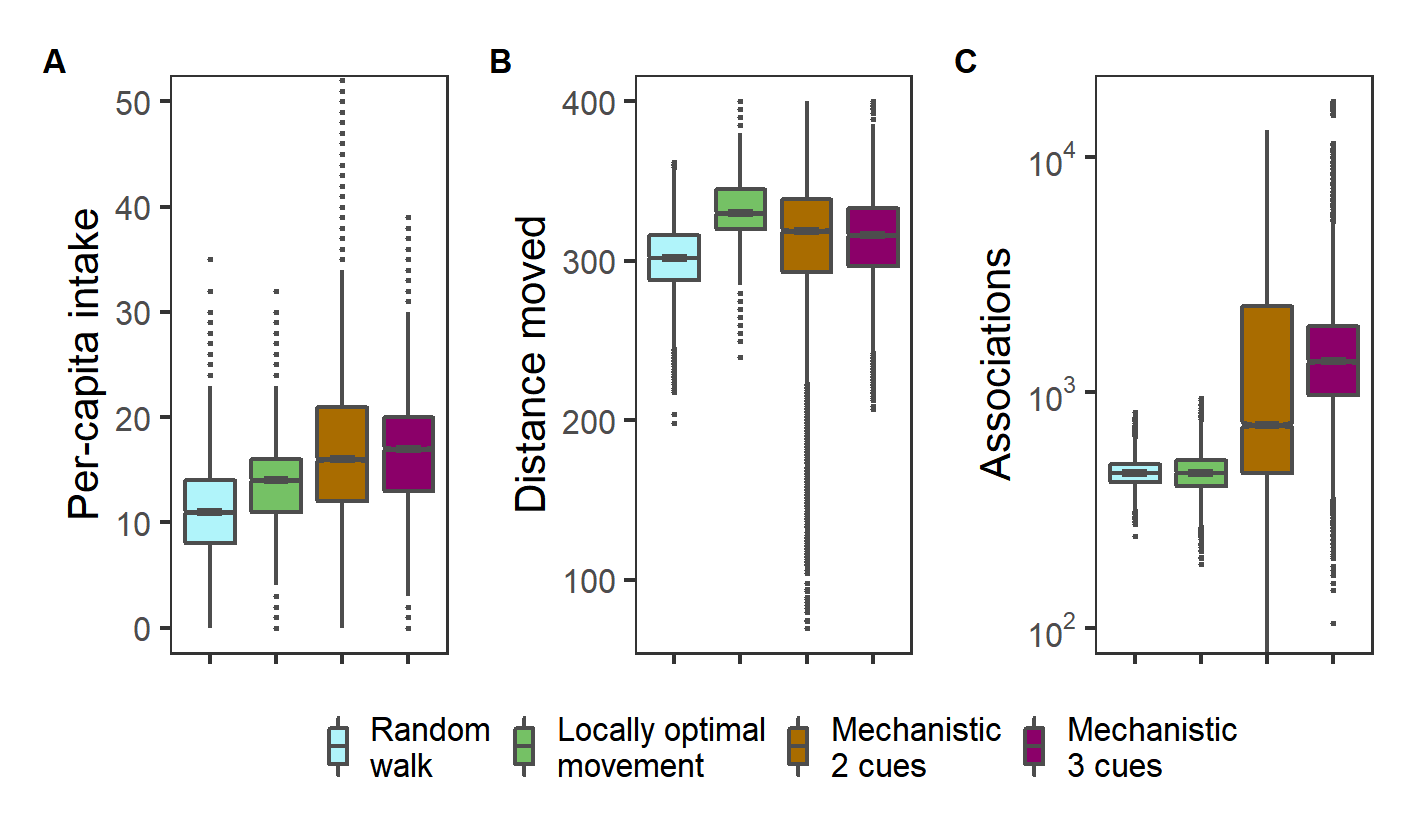
\includegraphics[width=0.95\linewidth]{figures/introduction/fig_case_study_ecological_outcomes.png}
    \caption{
        \textbf{Population ecological outcomes resulting from four types of movement strategy.}
        \textbf{(A)} In \textit{scenario 1}, individuals moving randomly across the landscape had expectedly lower per-capita intake than individuals moving in a locally optimal way (\textit{scenario 2}).
        When individuals selected their movement step based on heritable movement preferences for food items and conspecific competitors (\textit{scenario 3, `mechanistic 2 cues'}), after only 100 generations of natural selection for adaptive movement preferences, scenario 3 populations had a higher intake than ostensibly locally `optimal' movement.
        Allowing individuals to differentiate between current and future competitors (non-handlers and handlers, respectively; \textit{scenario 4, `mechanistic 3 cues'}), improved individuals' intake by a small amount, suggesting that adding information sources likely has diminishing returns, and that relatively simple step-selection movement strategies may suffice on even complex, fluctuating resource landscapes.
        \textbf{(B)} Surprisingly, locally optimal movers also moved more than random walkers, with no apparent trade-off between movement and intake.
        Individuals in scenario 3 moved less than those in scenario 2 (locally optimal), but still more than random walkers. Individuals in scenario 4 moved about the same as those in scenario 3, suggesting that being able to perceive neighbours' foraging status does indeed lead to more efficient movement strategies (i.e., more intake for similar movement).
        \textbf{(C)} Movement implementations strongly influenced individuals' associations (based on proximity), with step-selection based movement leading to many times more associations than random or locally optimal movement. Surprisingly, individuals in scenario 4 had many more associations than in scenario 3; this shows an unexpected difference that could have substantial consequences for the outcomes of social processes such as the transmission of animal culture or infectious pathogens.
    }
    \label{fig:demo_compare}
\end{figure}

I found that all 20 replicates of scenario 3 models showed that populations converged to a similar movement strategy within only a few (100) generations.
This strategy was to primarily prefer moving towards food items, while having a small preference or avoidance of potential competitors.
The `evolved' scenario 3 individuals had better ecological performance than their ancestral populations (which I consider the first generation, G = 1), taking in more food items on average, and moving less.
Indeed, these populations outperformed both the random walk and locally optimal movement implementations as well.
Adapting their movement strategies to the landscape also affected the social structure of scenario 3 populations --- there were fewer isolated individuals, more spatial clustering, and consequently, individuals encountered more unique conspecifics on average (higher mean degree; Fig.~\ref{fig:demo_networks}).

Individuals evolved after 100 generations in scenario 4 had mostly evolved a movement strategy that I describe as `handler tracking', i.e., having a preference for successful neighbours handling a food item ($sH >$ 0), but avoiding unsuccessful neighbours that were still searching for a food item \citep[$sN <$ 0;][]{gupte2021a,gupte2022c}.
% This is similar to the scenario 2 `locally optimal movement' strategy, and allows individuals to avoid areas with many potential competitors, and thus a lower potential intake.
Importantly this strategy allows individuals to use indirect social information \citep{dall2005,spiegel2016a}, in the form of the positions of successful neighbours, to find resource clusters --- even when these clusters are not immediately perceptible (due to earlier depletion).

Consequently, scenario 4 individuals outperform all three previous scenarios' individuals by having a higher mean per-capita intake (Fig.~\ref{fig:demo_compare}; in some cases, substantially higher).
This naturally leads to the conclusion that the resource landscape in scenario 4 is more depleted than in the three previous scenarios.
While not shown here, scenario 4 individuals after 100 generations of selection, also outperform scenario 4 populations that have not undergone selection (i.e., their ancestors), demonstrating the difference that adding evolutionary dynamics makes even to a mechanistic, habitat selection model.

Scenario 4 individuals' evolved use of social information on the potential locations of resource clusters also leads them to have more spatial associations with conspecifics --- indeed, up to three times as many as in the random walk and locally optimal movement models (Fig.~\ref{fig:demo_compare}).
These associations likely occur at or near resource clusters, leading to substantial spatial-social clustering in the final generation of scenario 4 populations (Fig.~\ref{fig:demo_networks}); and scenario 4 individuals across replicates associated with more individuals than in scenarios 1, 2 and 3.
Spatial-social structure in animal populations can have important consequences for a wide range of processes and phenomena in animal ecology, including the transmission of animal culture as well as the spread of infectious pathogens \parencite{romano2020,romano2021,cantor2021}.
The class of models I advocate are thus well suited to investigating questions around the emergent structure of animal societies (see Chapter~\ref{ch:pathomove} for more on this).

\begin{figure}[h]
    \centering
    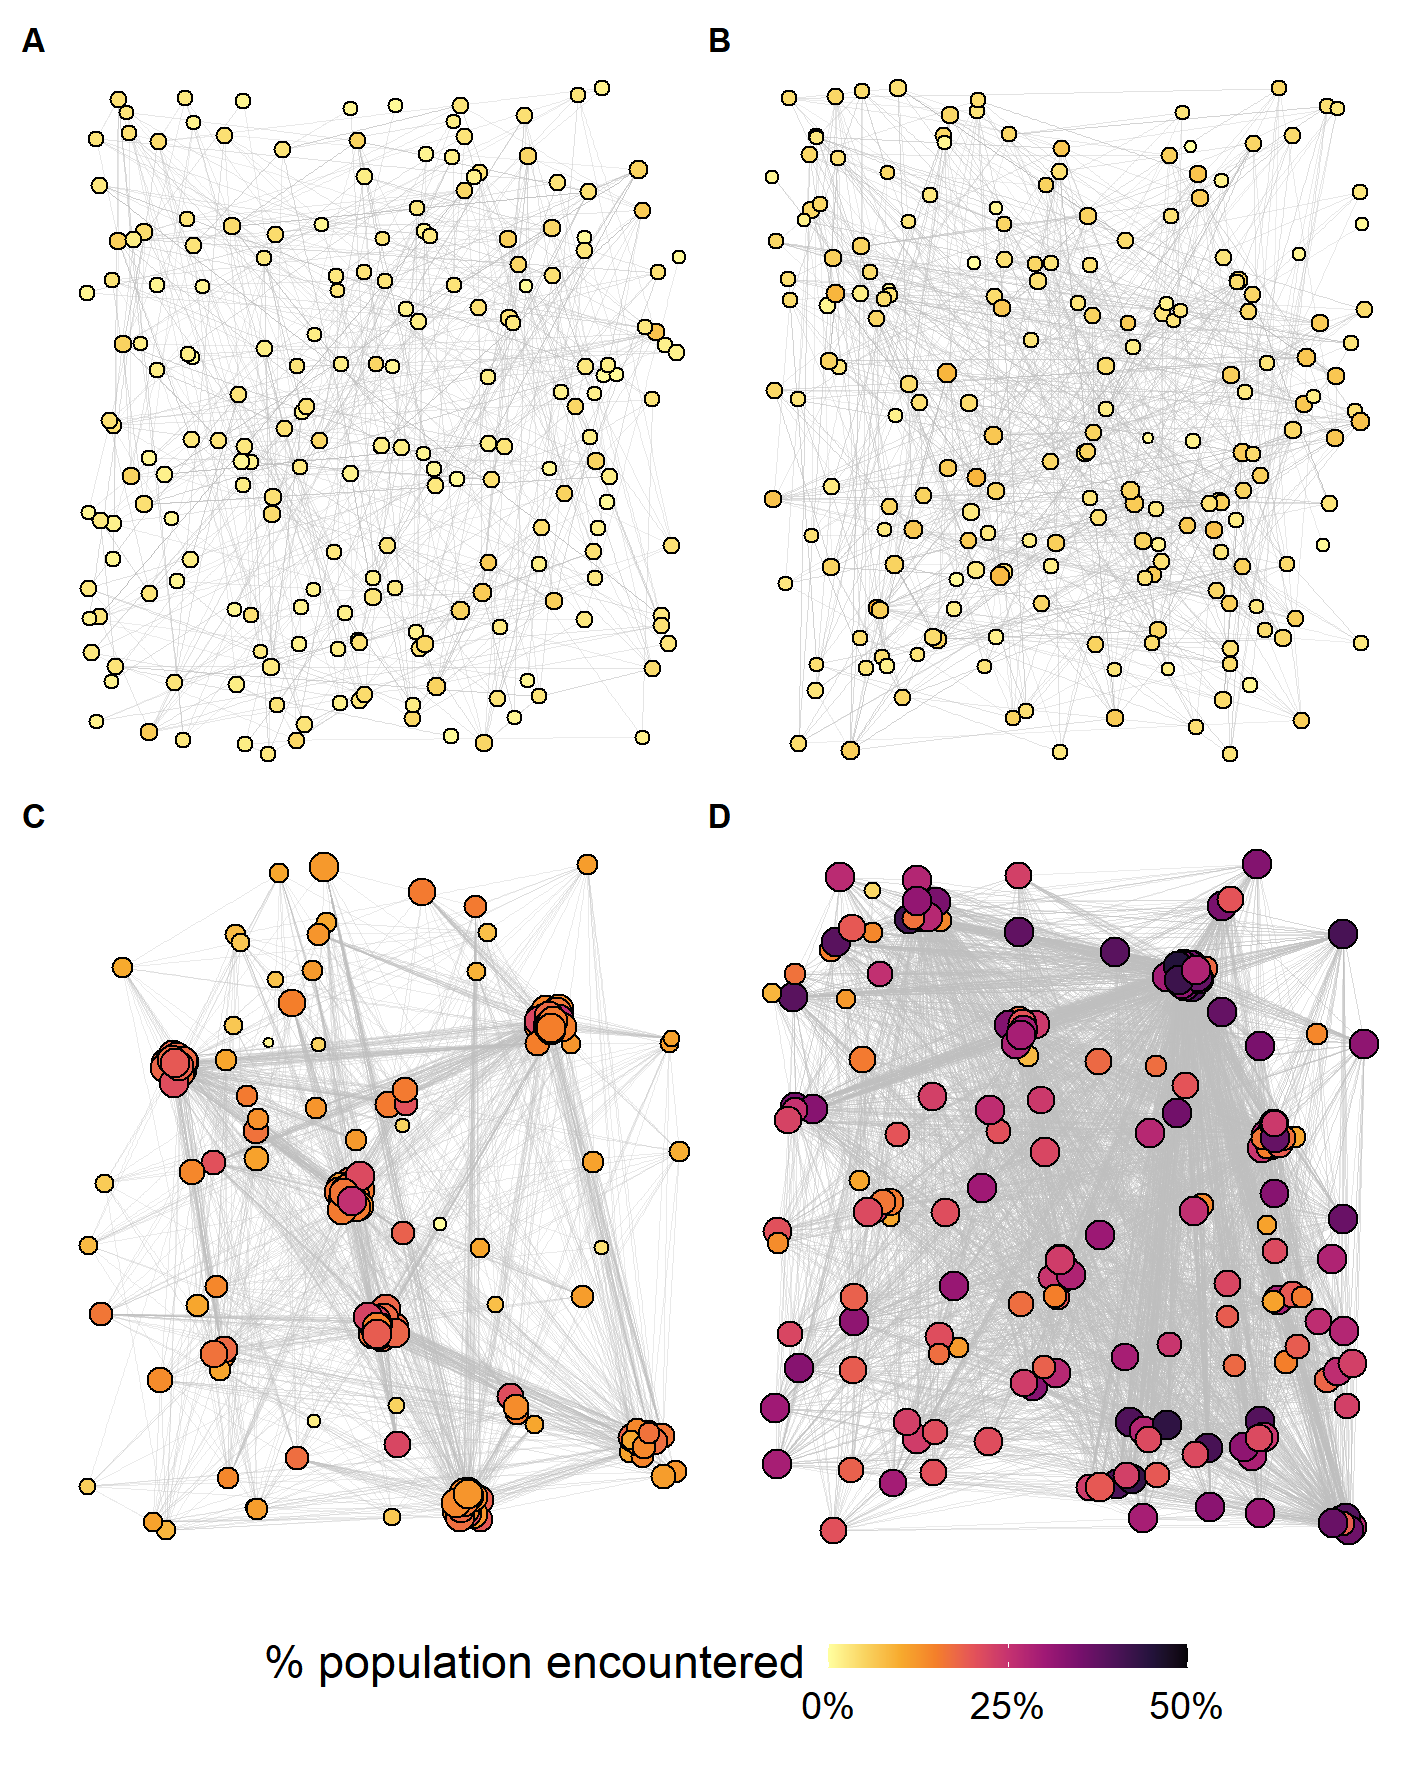
\includegraphics[width=0.9\linewidth]{figures/introduction/fig_networks.png}
    \caption{
        \textbf{Different movement strategies lead to substantially different patterns of spatial-social associations.}
        Individuals moving randomly (\textbf{A}: scenario 1), or in locally optimal ways (\textbf{B}: scenario 2) have sparse social networks, with individuals spread out over the simulated resource landscape.
        Most individuals have a low degree, i.e., few unique social partners.
        \textbf{(C)} In contrast, individuals making step-selection based movement decisions based on two cues (food and competitors; scenario 3) have much more spatially clustered networks, with a substantially higher mean degree (more unique social partners).
        Over 100 generations, scenario 3 individuals are selected for their preference for food items, and the resulting populations form networks that are also clustered, but with strong connectivity between clusters, and more unique partners overall.
        \textbf{(D)} A similar dynamic is seen in scenario 4, where most individuals still avoid immediate competitors (non-handlers), leading to more dispersed populations than scenario 3, though with strong links between nodes.
    }
    \label{fig:demo_networks}
  \end{figure}

\subsection*{Visualising and Interpreting Evolved Variation}

In scenarios 3 and 4, individuals' movement preferences (their weights for local environmental cues) may take any numeric value.
It is the combination of these weights that altogether forms each individual's movement strategies; this approach has been referred to as the `behavioural hypervolume' approach when applied to step-selection coefficients estimated from real animal tracking data \parencite{bastille-rousseau2019}.
One challenge in encoding behavioural strategies in this way is interpreting the evolved variation in strategies, if any.
A key step in doing so is exploratory visualisation --- the evolved movement preferences can be plotted in relation to each other to check for any obvious clusters.

Here, I would caution that conceptual individual-based models (and step-selection functions fitted to empirical data) may have to deal with a large number of model parameters \parencite{mueller2011}, or function coefficients \parencite{bastille-rousseau2019}.
This makes clustering and interpreting these individual-level attributes a challenge, requiring complex classification approaches \parencite{bastille-rousseau2019}.
This challenge is a powerful incentive to keep conceptual models' step-selection calculations as simple as possible.

\begin{figure}[h]
    \centering
    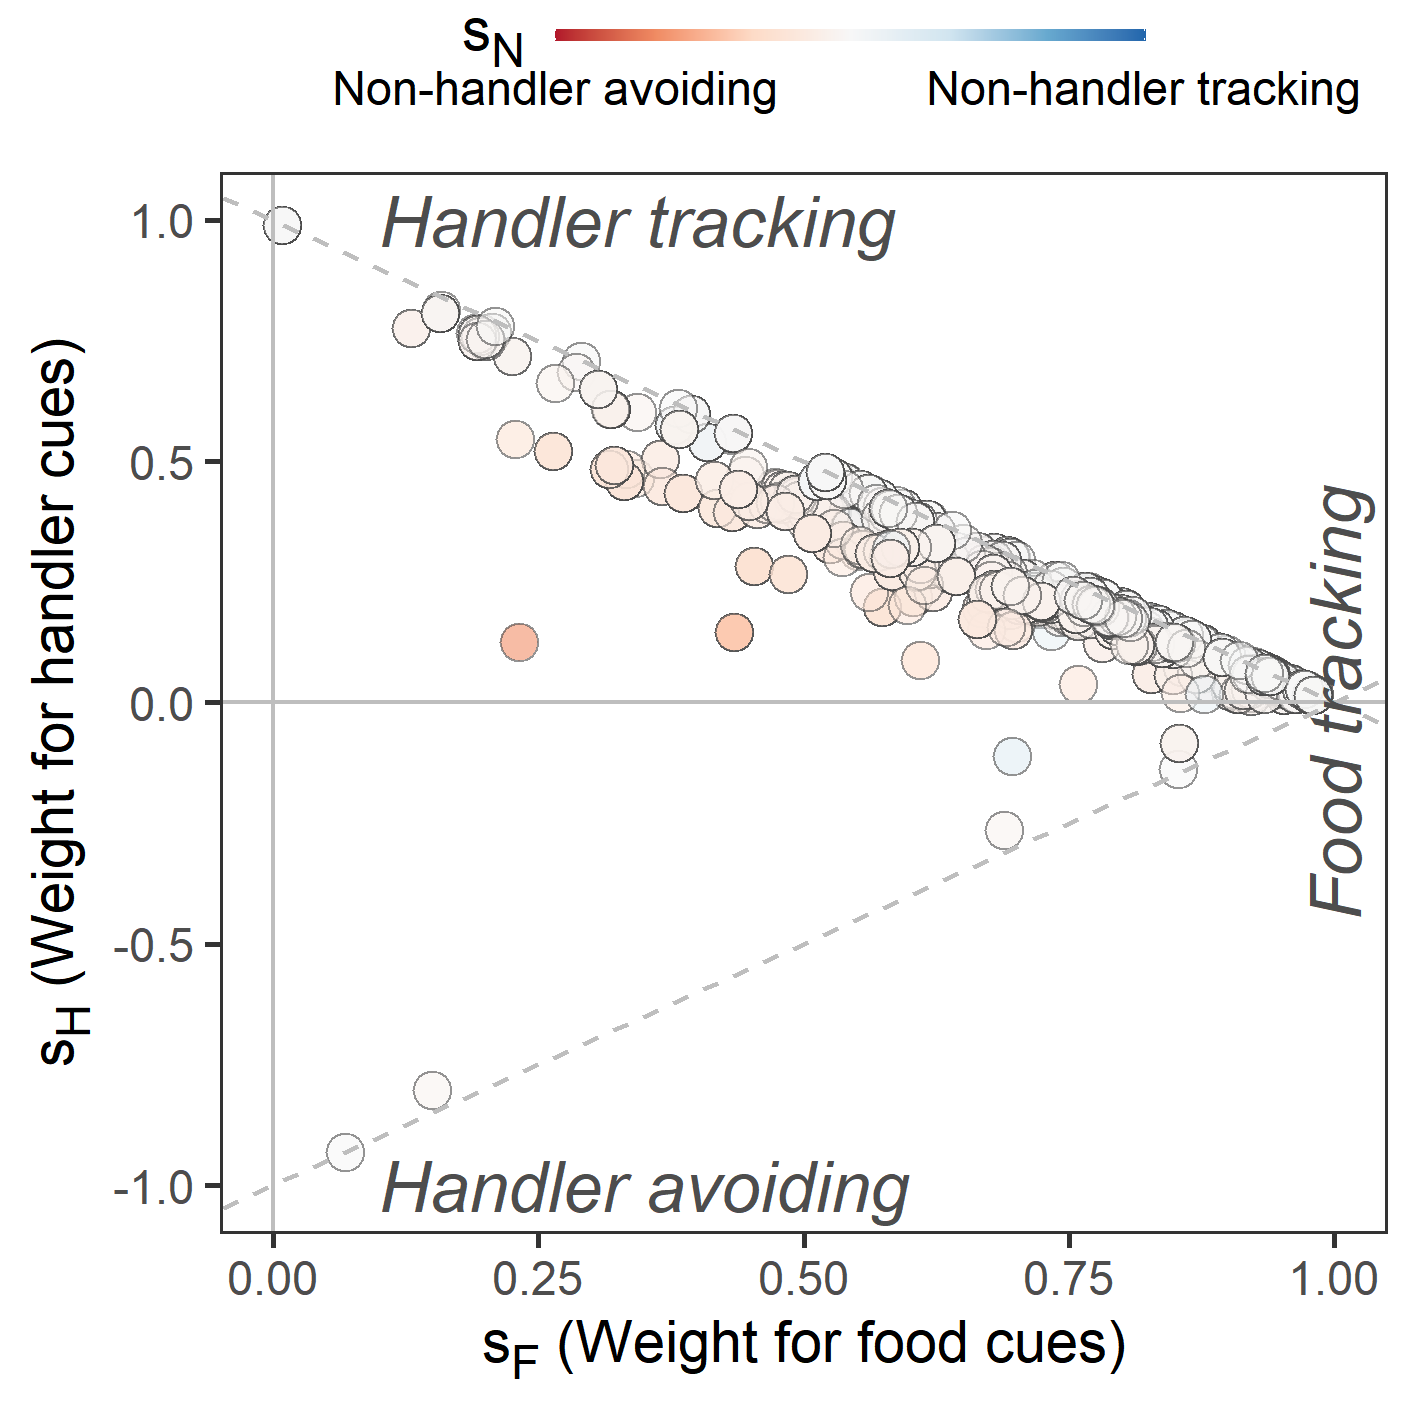
\includegraphics[width=0.7\linewidth]{figures/introduction/fig_hypervolume.png}
    \caption{
        \textbf{Evolved variation in step-selection movement strategies revealed by simple visualisation of evolved cue weights in scenario 4.}
        Plotting the scaled values of the heritable movement preferences (weights for local environmental cues) in a trait space bounded by [-1, +1] can reveal evolved individual variation in movement strategies. Here, most individuals lie along a behavioural spectrum: on one end ($s_F \approx$ +1.0), some individuals' movement decisions are mostly influenced by differences (if any) among food item counts at the potential destinations. On the other end ($s_H \approx$ +1.0), some individuals prioritise moving towards locations where there are many handlers.
        These patterns emerge spontaneously as results of natural selection from the simple mechanisms encoded by the model, without being forced by the modeller to represent any specific phenomenon. Yet they can be interpreted as showing the evolution and maintenance of individual variation, and especially of a broad mixture of producer-scrounger foraging strategies \parencite{beauchamp2008}.
    }
    \label{fig:demo_hypervolume}
  \end{figure}

In contrast, in my conceptual models, cue weights can be readily plotted in three dimensional space (with scenario 3 requiring only two dimensions for $s_F$ and $s_C$).
Here, I show how the three-weight individuals of scenario 4 (with $s_F$, $s_H$, and $s_N$) can be represented in a convenient figure: with $s_F$ and $s_H$ as the X and Y axes respectively, and the weight for non-handlers $s_N$ represented by a diverging colour scale (Fig.~\ref{fig:demo_hypervolume}).

The interpretation of this figure, which also helps with similar figures in chapters~\ref{ch:kleptomove} and~\ref{ch:patternprocess} is as follows.
Each point on the figure represents a single individual.
Each individual is plotted in a three dimensional space (colour representing position in the third dimension); this is \textcite{bastille-rousseau2019}'s behavioural hypervolume.
Each individual's position is calculated by scaling each of its cue preferences (say, $s_i$) by the sum of the absolute cue preferences: $\text{scaled}~s_i = s_i / (\Sigma |s_n|)$.
This means that regardless of the number of cue preferences (in this case, three), all axes are bounded by [-1, +1].
The regions individuals can take in the two primary axes is bounded by the dashed lines.

Individuals that lie towards the extremes (-1 or +1) of any axis should be interpreted as making their movement decisions primarily based on that particular cue.
For example, in Fig.~\ref{fig:demo_hypervolume}, many individuals have values of $s_F$ close to +1.0, indicating that they `assign' food item cues the highest, and indeed nearly all the weight when making movement decisions.
Another perspective on this is that for such individuals, the combination of cue values and the individuals' weight for them (e.g. $s_N \times N$) is often less than $\epsilon$, i.e., their sensitivity to the cue is on the order of their perception error --- not of great importance.
This same interpretation applies to individuals' position on the colour scale; extreme values indicate a strong preference or avoidance of the relevant cue (here, $s_N$).

Interestingly, plotting individuals' evolved movement strategies in this way reveals that there is a substantial amount of variation among individuals.
Indeed, individuals appear to occupy a spectrum between prioritising only food item cues (high $s_F$) and only handler cues (high $s_H$).
More rarely, some individuals' position indicates that they have a strong avoidance of non-handlers.
In this model, this suggests that a broad range of movement strategies can and does coexist, neatly demonstrating that behavioural variation can arise spontaneously from simple mechanistic assumptions in this class of models.
Similar figures in chapters~\ref{ch:kleptomove} show how strong correlations can arise between movement strategies as shown here, and other behavioural strategies.

% \subsection*{Emergent Model Properties: Consequences for Disease Transmission}

% To examine the consequences for disease ecology, I began by constructing social networks by recording individuals' pairwise associations (distance $<$ perception range) in all four scenarios \citep{farine2015}.
% I ran simple epidemiological models with SIR assumptions over the social networks emerging in each scenario \citep[25 replicates per network; 1 network per scenario replicate][]{white2017,csardi2006,bailey1975}, with a hypothetical disease (transmission probability $\beta$ = 2.0, recovery probability $\gamma$ = 1.0; see Fig.~\ref{fig:sir}).
% Between the non-mechanistic scenarios, the disease spread more rapidly through networks arising from the locally optimal movement model, than the random walk model.
% In scenario 3, the disease spread much more rapidly through the population after selection for movement preferences (G = 100), than through the ancestral population that had not undergone such selection (G = 1), despite both populations being similarly spatially clustered.
% This is not unexpected as initially (G = 1), there are a number of individuals that avoid potential competitors ($s_C <$ 0), and this could hinder transmission in comparison with their descendants, fewer of which are similarly isolated.
% Importantly, the unevolved mechanistic movement implementation had a lower infection peak than the random walk and locally optimal movement implementations.
% A model beginning with diverse movement strategies, and not including an evolutionary component when implementing mechanistic movement \citep[such as][]{white2018}, would correctly conclude that mechanistic movement implementations differ from more mainstream movement modelling approaches in epidemiological outcomes, but crucially miss that this difference is that a disease would spread much more rapidly through the population.
% Scenario 4 obtains a similar result --- populations adapted to their landscape cluster together, which allows a disease to spread even faster through their network than in scenario 3.

% \begin{figure}[!h]
%     \centering
%     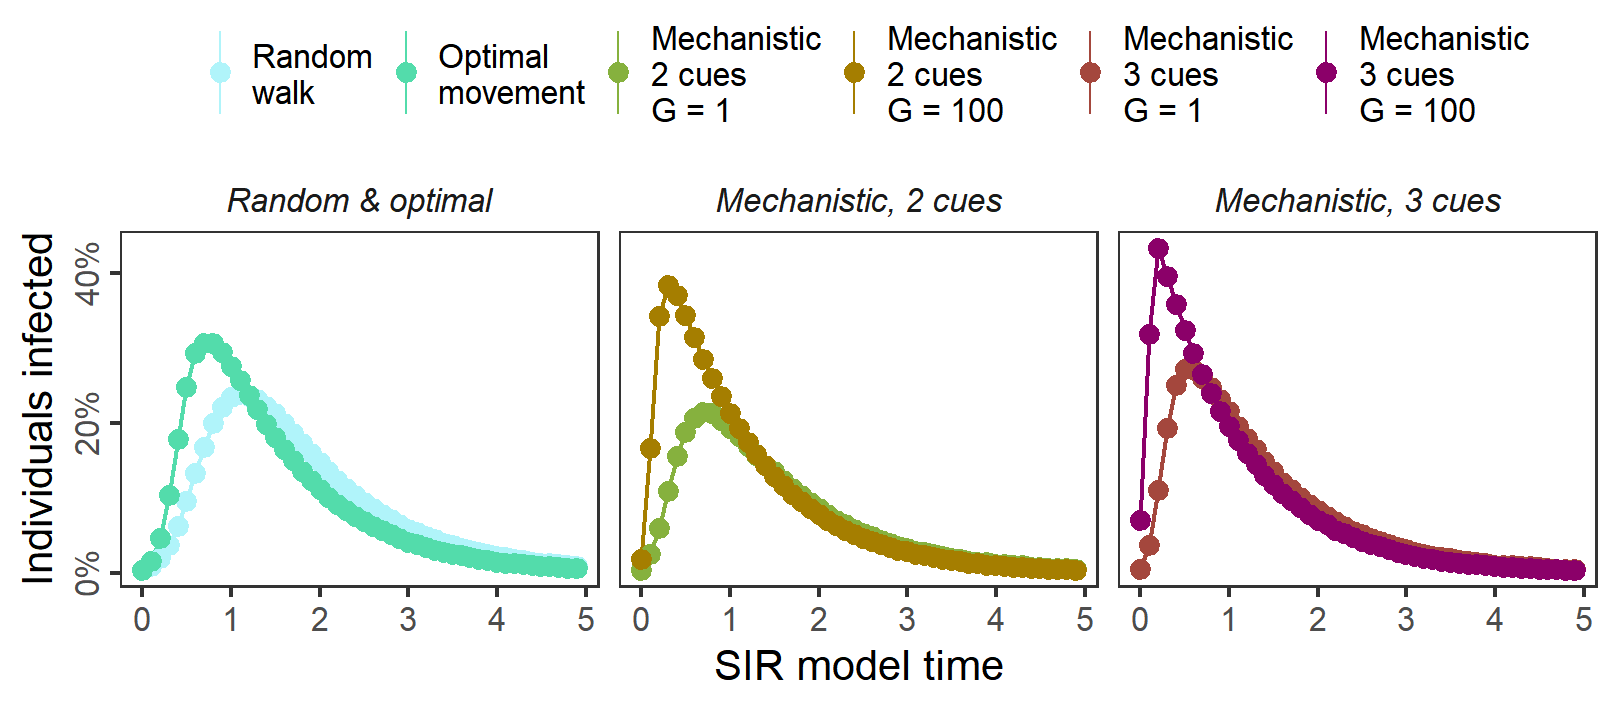
\includegraphics[width=0.9\linewidth]{figures/introduction/fig_cs_2_2.png}
%     \caption{
%         \textbf{Case study 2: Effect of movement implementations on the outbreak of hypothetical disease.}
%         Modelling a disease outbreak using a simple SIR model conditioned on the social networks of each population (e.g. as shown in Fig.~\ref{fig:demo_networks}) shows that how movement is implemented in models can strongly influence epidemiological conclusions (disease transmission rate $\beta$ = 2.0, recovery rate $\gamma$ = 1.0).
%         \textbf{(A)} The hypothetical disease spreads more rapdily through \textit{scenario 2} than \textit{scenario 1}, as scenario 2 networks are somewhat better connected. This is likely because locally optimal movement is better at leading individuals towards resource clusters where they must associate with conspecifics while feeding.
%         \textbf{(B)} Modelling movement as mechanistic step-selection based on preferences for local cues (\textit{scenario 3}: mechanistic, 2 cues) leads to drastically different conclusions depending on whether the model includes an evolutionary component. Diseases spread less rapidly through ancestral populations with a diversity of movement strategies, than through populations moving optimally or even randomly.
%         However, after 100 generations of selection, the population has primarily social agents that are strongly inter-connected, leading to very rapid disease outbreaks.
%         \textbf{(C)} Disease dynamics are similar in \textit{scenario 4} (mechanistic, 3 cues): the spread of disease through initial networks (G = 1), is not representative of the spread through populations that have undergone selection (G = 100).
%     }
%     \label{fig:sir}
%   \end{figure}

% Overall, individual-based models offer the potential for more realistic social networks to emerge, with the expectation of more robust epidemiological insights from these networks \citep[][]{lunn2021}.
% The development of spatially explicit movement-disease models allows both movement and disease transmission dynamics to be modelled explicitly \citep{white2018b,white2018,scherer2020,gupte2022c}.
% However, network models conditioned on emergent social networks allow multiple pathogen scenarios to be run on the same network, saving computational time, and they also enable comparison with empirical work in the disease ecology of moving animals \citep{wilber2022}.
% The importance of network formation processes in epidemiological modelling is already well known \citep[][]{white2017,wilber2022}.
% My example model demonstrates how social networks emerging from individual-based movement models are sensitive to the modelling of the movement process, and how model details can affect predictions about disease outbreaks, and animal spatial-social ecology generally \citep{webber2018,webber2022}.
% Furthermore, including evolutionary dynamics in combined movement-disease models can reveal surprisingly rapid evolutionary transitions in social movement strategies that make populations more robust to the spread of pathogens (see Chapter~\ref{ch:pathomove}).

{ \begin{center} \barfont{-.-} \end{center} }

\end{interludeenv}
\endgroup
